%!TEX root = main.tex

\documentclass[../main.tex]{subfiles}

\begin{document}

\chapter{Sound Design and Controlling Parameters}
Fill me in later

\section{Alternate Architecture Considerations}
\section{Tuning Parameters}
Explain how DC blocker is different than not using absolute value function in noise source
\subsection{$T_{60}$}
$T_{60}$ is not full described in the original \citetwo{pakarinen_virtual_2008} paper. This paper describes the type of string as determining both the decay time as well as duration and an individual noise pulse. Given that the noise pulses have an exponential amplitude envelope, ultimately only one of these are needed as the decay time and duration can be derived from each other. There is no specification as to how the decay rate is specified either, so the $T_{60}$ value was chosen as this is a widely known and standardized parameter for reverberation time. It has been adapted here to represent the amplitude envelope's time until it decays 60 dB from its original value (and does not correspond to any sort of reverberation).

The implementation of the algorithm as described in \citetwo{puputti_real-time_2010} does not clearly define how the decay rate and pulse length are specified as well. Their implementation is more akin to the guqin model (\citetwo{penttinen_model-based_2006}) or noise burst approach where the stacking of the impulses is not allowed to occur in an unrestrained fashion. This makes the signal less harmonic and more noise like as the fundamental repetition of the slide/winding collision impulse response is not allowed to occur in a more sonically meaningful way.

There is also a question as to the physical interpretation of the noise pulse as it has been described originally in \citetwo{pakarinen_virtual_2008} and implemented in \citetwo{puputti_real-time_2010}. Figure \ref{fig:noise_pulses} illustrates the noise pulses as originally described. It is clear here that the noise pulses do not take on negative values. This is also reflected in Figure B.21 in \citetwo{puputti_real-time_2010} where an \emph{abs~} block has been applied after the \emph{noise~} in the PD implementation.

\begin{figure}[h]
    \centering
    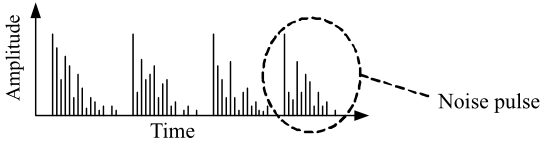
\includegraphics[scale=.75]{./images/pictures/noise_pulses.PNG}
    \caption{Image of noise pulses take from \citetwo{pakarinen_virtual_2008}}
    \label{fig:noise_pulses}
\end{figure}

The physical interpretation of a noise burst is meant to represent the impulse response of a single slide/winding impulse. However, what does an impulse response which does not take on negative values here indicate? This would seem to indicate that there is no oscillatory motion and the signal only decays. Without oscillatory motion, how can there be any sort of wave motion? Equation 1 from \citetwo{pakarinen_analysis_2007} indicates that the noise pulse is meant to represent $f(t)$, which given the existence of the modes would imply some sort of a negative values. $f(t)$ represents the force that an infinitesimally small cross-section of the string would experience over time after having a collision. Additionally, this also adds a DC component to the noise source which can build up in the DWG due to the coupling between the longitudinal and transverse motion.

\subsubsection{Tuning}
Attempts were made to empirically measure the $T_{60}$ value, however the measurement equipment was not sufficiently low noise to allow for a meaningful result to be calculated. Instead, an attempt will be made to determine the correct value based on trying to match the spectrograms where were measured. The crucial component to understanding this observing the relationship between the decay rate and the firing rate. The longer the decay rate is, then the lower the firing rate needs to be in-order to have the impulse responses overlap. The more the noise pulses overlap, the more "noise like" the signal becomes due to the build up of energy. If this build up is too much then the harmonic component of the signal is obscured. Signal-to-noise ratio could be an apt term to describe this, however the standard definition of this implies that the "noise" component is unwanted. Given that the "noise" component is useful as a stimuli for the longitudinal-mode filters which follow it in the CSG', the desirability of "noise" is ultimately subjective as it is a creative decision by the person playing the synthesizer. The $T_{60}$ parameter ultimately controls the haromonicity to noise transition frequency for $f_c[n]$.

\section{Waveform Initialization}
Two different types of noise were experimented with for specifying different initial conditions for the DWG's buffer: white and pink noise. Each noise type has a different properties regarding its frequency content. White noise contains equal frequency content across the spectrum, whereas pink noise has a spectrum where there is equal energy per octave. Accordingly, pink noise is skewed more towards the lower end of the spectrum while white noise contains more energy at the upper end for a specified sampling rate. Experiments were done with both types of noise. There is an audible difference between the two, where the white noise generated signal contains more definition/clarity in the attack. Intuitively this makes sense as the higher frequencies are necessary to create sharper transitions associated with a faster transient. The pink noise generated sounds have more of a ``warmer" sound due to their stronger low-frequency content and are more natural sounding. Pink noise was used in the \citetwo{puputti_real-time_2010} implementation while historically white noise has been used as illustrated by \citetwo{karplus_digital_1983}. 

TODO: Add sound examples with both types to illustrate the differences. Perhaps add spectrograms and snapshots of the waveform attack.

\subsection{Removing DC Component from String DWG}
In either case it is necessary to remove the DC component from the signal as it doesn't add anything to the sound's timbre and can cause issues with computations if it builds up too much in the digital waveguide structure. It is easiest to achieve this when the waveform is initialized in the memory where the digital waveguide is stored. The standard method of achieving this is by computing the mean of the buffer and subtracting this from the waveform. Given that the digital waveguide's length is distributed across three different components (an integer delay line, an interpolation filter and a loop filter) there is a question of where to store the initial waveform. Through experimentation is was determined that the integer delay line was the best place to achieve this. Fundamentally it is impossible to generate a waveform which has a non-integer number of samples, so this is the only buffer which is guaranteed to be able to be filled at any digital waveguide length. Additionally, the processing effects of the loop and interpolation filter are dynamic depending on the synthesis context and in cascade with each other so the effects of the interpolation filter have an impact on the sample which is stored in the loop filter.

In terms of the actual initialization, it is necessary to only initialize as many samples which correspond to the integer delay line's length for a particular digital waveguide length. Suppose that the data structure for the buffer has been set to have a maximum of 1000 samples but only 250 samples are required for the integer delay line. Only those 250 samples should be considered as those are the only ones which will get played out. The others will be overwritten as the algorithm computes output samples, so they would introduce an unwanted bias in the waveform. Contrary to white noise, pink noise is correlated with itself. So generating more samples than is necessary would ultimately not result in pink noise as the other samples would never be played. Beyond that, it would be necessary to remove the bias from the entire generated waveform, but given that part of it would never be accessed, an unwanted DC bias would be introduced into the component which is played out. This would be introducing the exact thing which we were trying to prevent.

TODO: ADD SOME PICTURES FOR THIS

\section{Control Signal Parametrization}
An attempt was made to synthesize the following musical segment.

TODO: INSERT FIGURE OF THE SLIDE LICK HERE

This example was also played and recorded to be able to compare the difference between the synthesized figures and the real playing examples. This occurred across multiple different parameters, but the primary one of interest was the accuracy in terms of the specified control signal. The goal of a musical synthesizer is to be able make make musical sounds (something which is fundamentally subjective), however one way of determining the ``musicality" of a synthesized sound would be to compare it to a recorded example.

Comparing an artificially constructed $L[n]$ to an extracted one is one way of doing this. This is true as there is only one control signal and ultimately one of the defining characteristics of slide guitar is that this can take on values which normally aren't achievable by frets. The recorded example was run through the YIN algorithm and its output is shown in figure \ref{fig:YINOutput}. The blue lines represent areas where the YIN estimation is most reliable, where the green is less reliable and yellow is the least reliable. The note attacks as well as decay at the end are less reliable as they contain less periodic content which is necessary to estimate a fundamental frequency.

\begin{figure}[h]
    \centering
    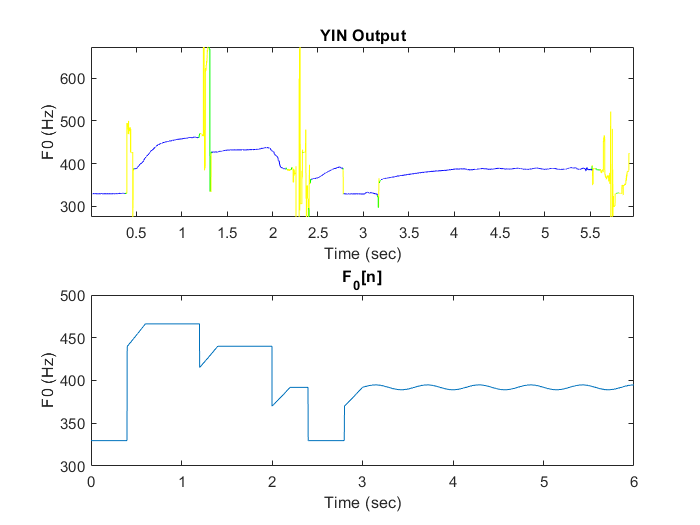
\includegraphics[scale=.65]{./images/plots/F0Compare.png}
    \caption{Comparison of Recorded Example vs. Synthesized Signal F0}
    \label{fig:YINOutput}
\end{figure}

The files being compared can be heard in \emph{GETFILENAME.wav} and \emph{GETFILENAME.wav}.

One of the main things to note is the transitions between notes are substantially more nuanced in the YIN analysis of the recorded playing example. This is due to the human element factor and the fact that no one person ever plays the performance the same way twice. Determining an algorithm which would match these curves would be quite a difficult task. It would be easier to just extract this signal and attempt to use it as a parametrization curve for the component.

The second plot in the figure illustrates the fundamental frequency which should be generated based on synthesis parameters specifed in the example. The slides were approximated by using the \emph{generateLCurve()} (ADD BACKGROUND INFO ON THIS FUNCTION) but by specifying that the slide is a one fret slide from below which has a duration of a 16th note. The results are something which sound very much like it was controlled and generated by a computer. The YIN output clearly indicates far more nuance in the different types of slide  approaches to notes as well as their articulations. An area of potential future research would be attempting to classify different sorts of slide articulations and algorithmically generating them. Another approach would also be developing an algorithm to cleanly extract the $L[m]$ signal from an recorded example to be able use it to control the algorithm. At points they seem logarithmic (i.e. first big slide from .5 to 1.25 sec), however given the myriad of ways in which articulations can be achieved via a slide, codifying one approach seems to be a poor decision.

The slide transitions are linear in the computed approach for some reason, even though the underlying algorithm has been specified to operate logarthmically. Although for small enough segments it is approximately linear and we are considering only a 1-fret slide in
from below over the course of a 16th note at 75 BPM. This note duration is approximately 47 milliseconds.

\end{document}